\noindent
The healthcare systems of the future will be highly decentralised, integrating home-, work- and environment-based monitoring into the hospital diagnostic systems, thus reducing costs and travel-associated risks while allowing patients to get better medical treatment (Figure~\ref{fig:dataExch}). As a consequence, medical data will need to be collected from a variety of sources and exchanged in a variety of ways, including over public networks that cannot be implicitly trusted. At the same time, we have more and more strict regulations about ownership and access rights for the patient data. Trans-national standards for data protection, such as GDPR~\cite{gdpr}, will need to be combined with local regulations, giving very strict rules about who is allowed to access what part of patient data. Complying with these rules while, at the same time, facilitating data exchange and analytics in decentralised way will be the main challenge for the future healtcare systems.

\begin{figure}[ht!]
    \centering
    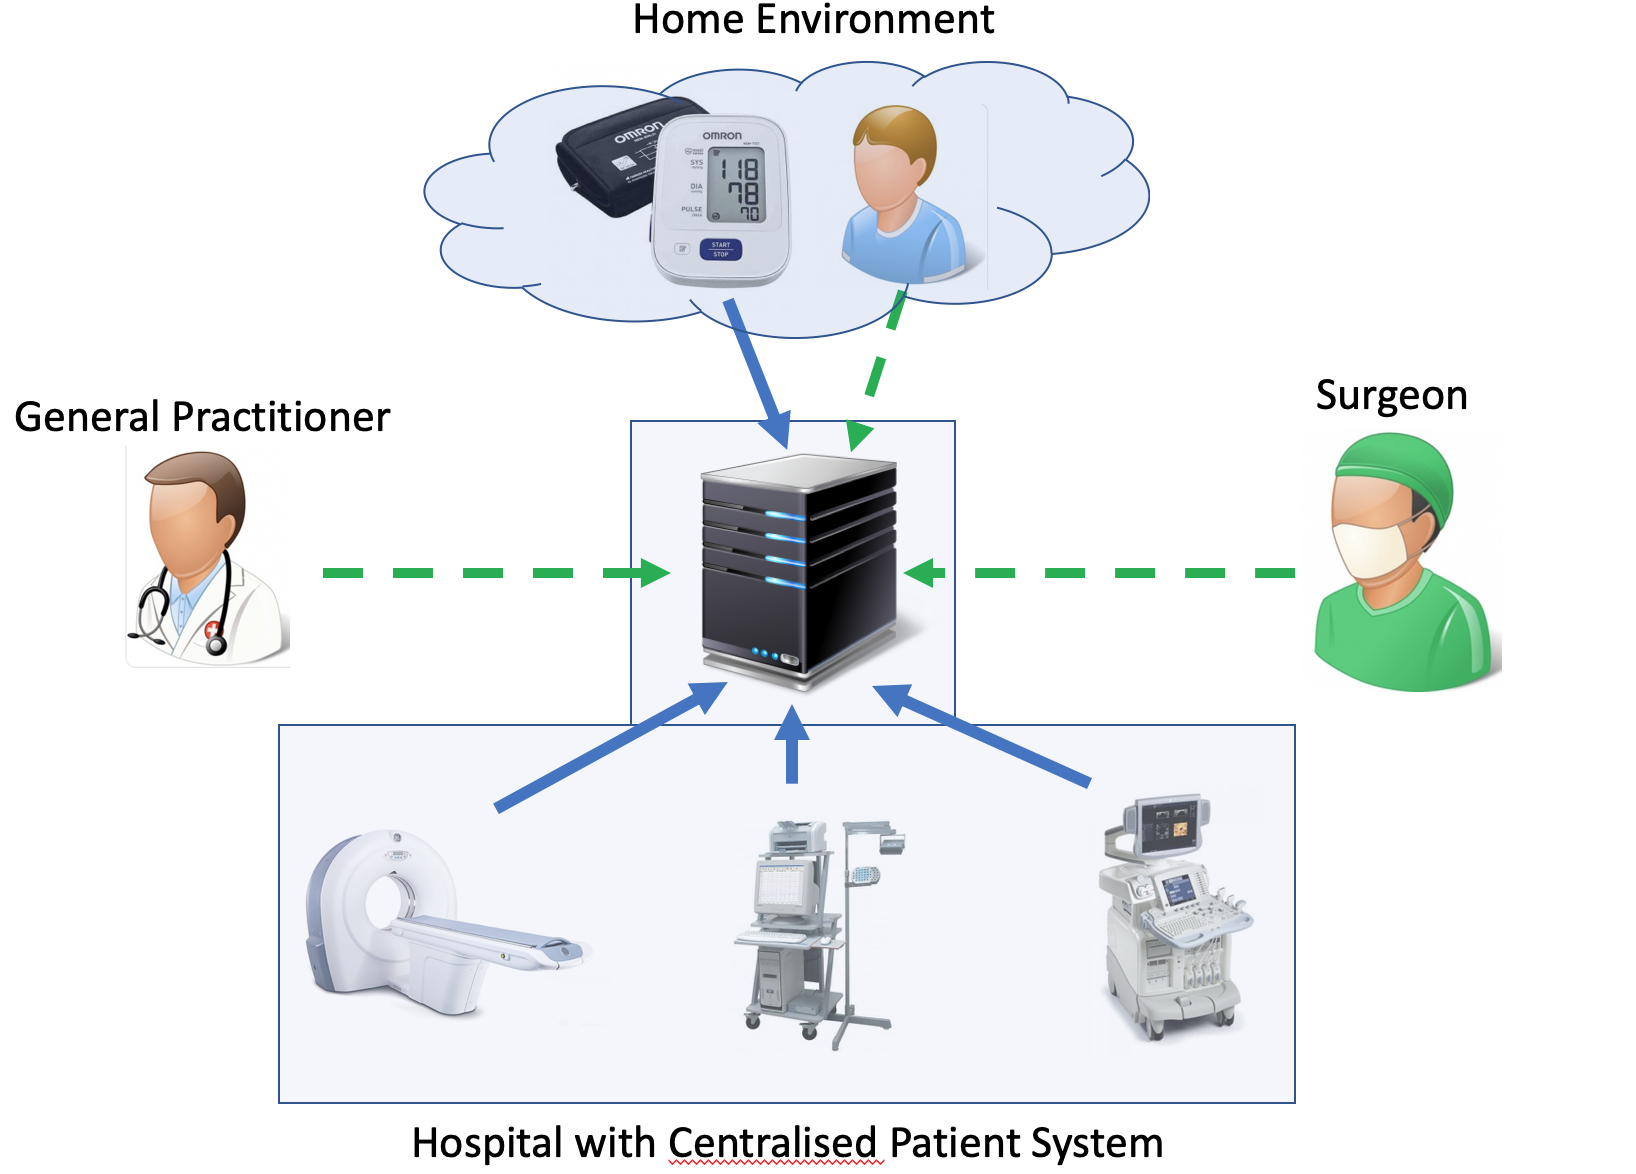
\includegraphics[width=70mm]{images/DataExchange.png}
    \caption{Data Exhcange in Modern Healthcare Systems}
    \label{fig:dataExch}
\end{figure}

In this paper, we describe a methodology that will be developed over the course of the ongoing \emph{Serums: Securing Medical Data in Smart Patient-Centric Healthcare Systems} EU H2020 project and that will address the issues of safe, secure and confidential storage, access, communication and analysis of the medical data in future-generation smart health centers. Our main goal is to put patients at the centre of future healthcare provision, enhancing their personal care and maximising the quality of treatment that they will receive, while securing trust in the security and privacy of their confidential medical data. To this end, we aim to develop a complete tool-chain that will ensure security and privacy of data over its whole lifetime, from collection and storage to the distributed analytics.

To reduce the scope of the paper, we restrict our attention to a subset of all \emph{Serums} technologies. We propose a universal format for patient records, the aim for which is to allow uniform representation of patient data across different use cases, and describe its implementation using the \emph{data vault} concept from data science. We also describe authentication and authorisation mechanisms to access these records, together with application of blockchain technology to control permissions and ensure only the allowed agents are allowed to access the relevant parts of patient records stored and processed within a \emph{data lake}. We then describe a novel, \emph{privacy-preserving} data analytics mechanisms to analyse the data, while making sure that the analytics model does not accidentally leak any sensitive information. Finally, we present the \emph{data fabrication} methodology that allows us to generate, based on strict format of the smart patient records and rules for dependencies between its elements, synthetic but realistic data that will be used for rapid development and stress-testing of the \emph{Serums} technologies.


This paper makes the following concrete research contributions:
\begin{itemize}
\item Contribution 1
\item Contribution 2
\item Contribution 3
\end{itemize}

\section{Background}


\subsection{Issues for Modern Health Care Centres}

\textbf{USTAN to write the first version}

\subsection{The Serums Project}

\textbf{USTAN to write the first version}

\section{Serums Tool-Chain For Smart Health Centre Systems}

\begin{figure}[ht!]
    \centering
    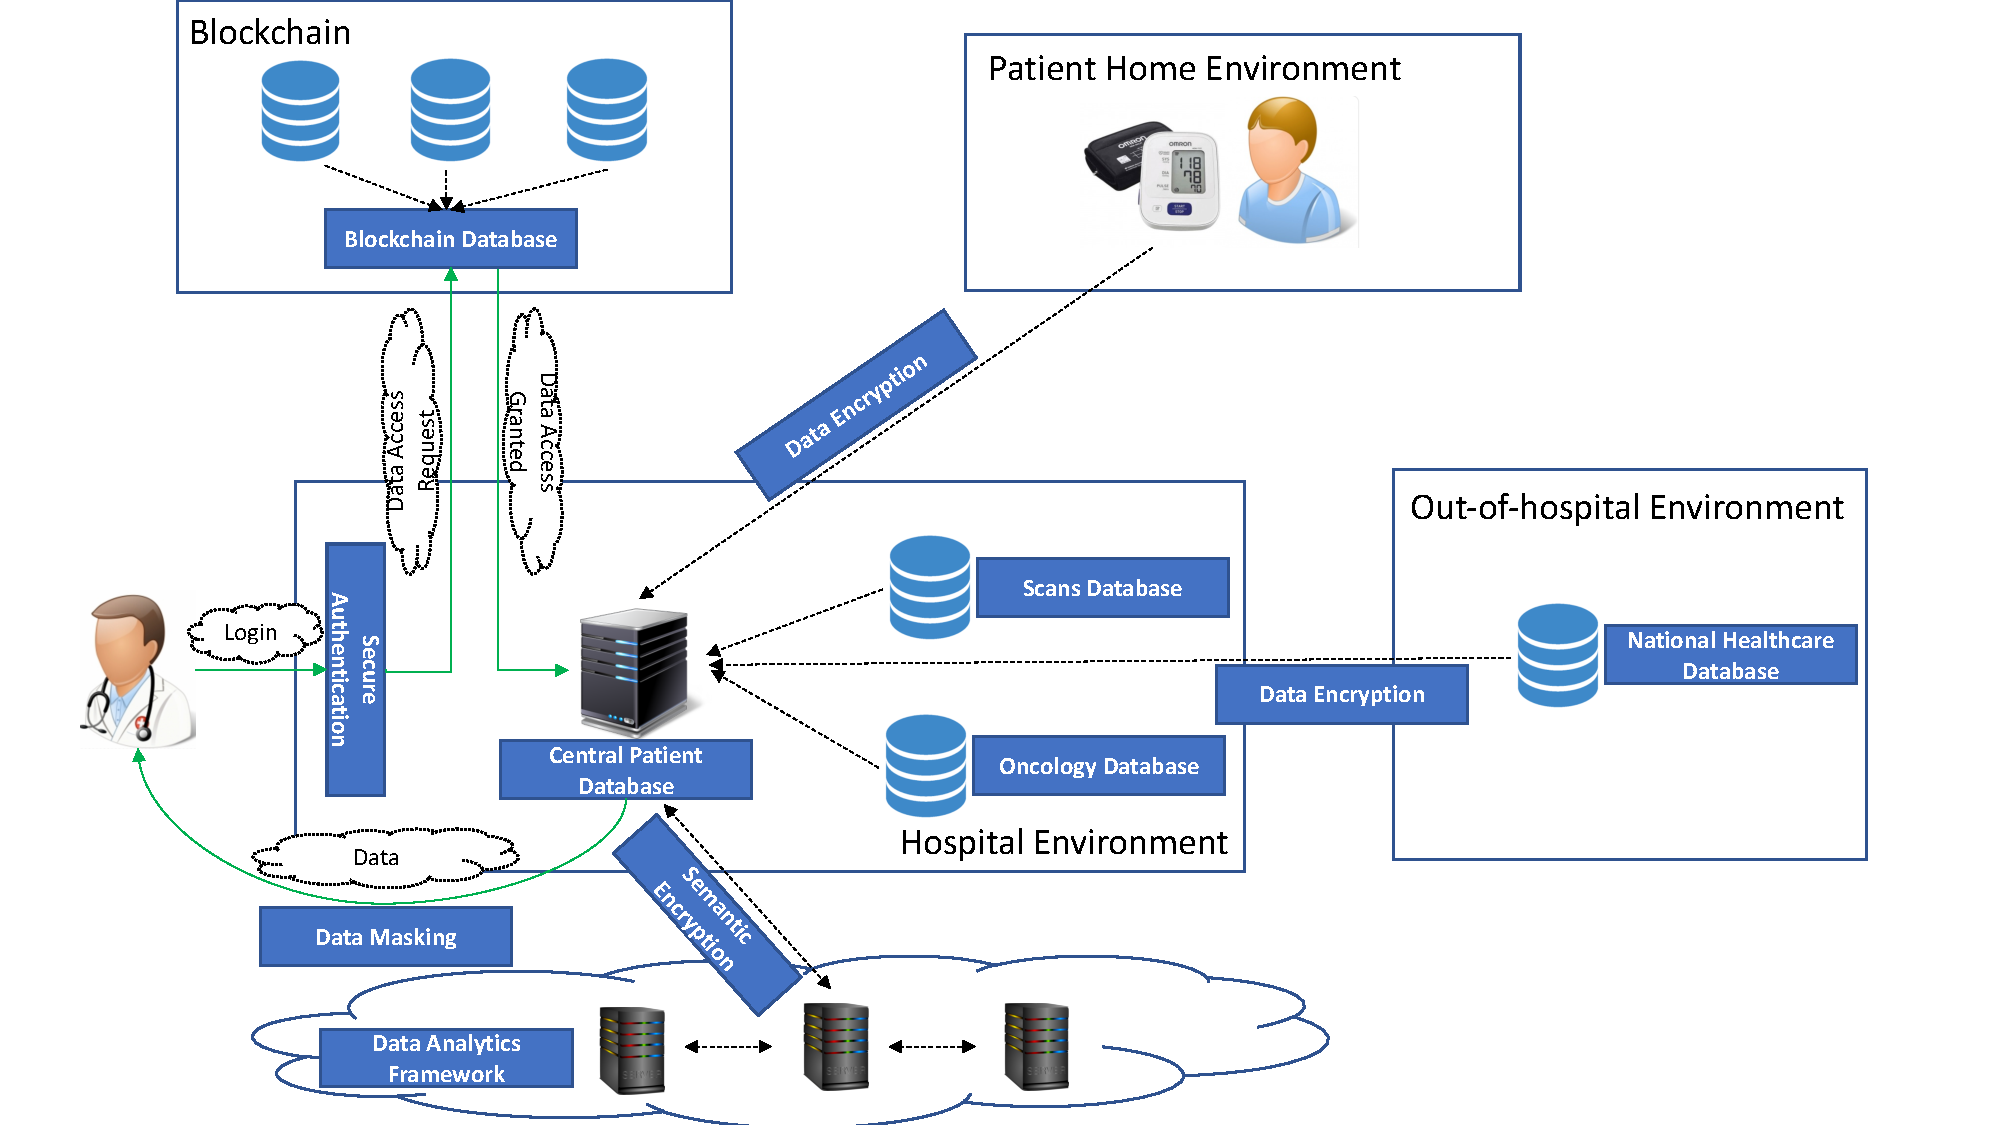
\includegraphics[width=90mm]{images/SerumsOverview.pdf}
    \caption{The overview of \emph{Serums} tool-chain}
    \label{fig:serumsTools}
\end{figure}

\noindent Figure~\ref{fig:serumsTools} gives an overview of the \emph{Serums} tool chain and the overall process of accessing and using the smart health centres that will be based on it. The core of it is the centralised data lake with various databases that forms the \emph{smart patient records} (see Section~\ref{sec:smartrecords}). These records contain all information about the patients, from static information such as date of birth, gender and contact information, to vital information such as weight, body mass index, allergies, to dynamic information about treatments and examinations. While we assume that all the records are stored in one location, the data that they refer to might reside in different distributed data storage technologies, i.e.~the records can contain \emph{remote pointers}. Some of the data for the records will be collected from within the healtcare system over trusted networks, while the other may be collected from the personal health monitoring devices from patient's home or workplace. The latter data may need to be sent over mistrusted networks and, hence, needs to be secured using \emph{data masking and encryption} mechanisms.

For the purposes of developing and testing the complete infrastructure, it might be preferable to use \emph{synthetic} instead of real patient data, to avoid any privacy and security concerns. \emph{Data fabrication} (See Section~\ref{sec:datafabrication}) technology allows us to rapidly generate large volumes of the data that is the same in terms structure as the real data, but the fields of which are synthetically generated. The strict format of the smart patient records, with formally defined rules about the values of each field, relationships between different fields and well-formulated data interaction rules, allows this process to be performed automatically. 

The data is accessed using \emph{secure authentication and authorisation} mechanisms (see Section~\ref{sec:authentication}). \textbf{VJ: Add a few sentence of why we need this and how it works}. As an additional layer of protection, the \emph{blockchain database} serves to control the access rights of the authorised agents to the patient records. Different agents will have different level of permissions, according to GDPR and other regulations. For example, the patient will have full access to its record, while any specialist will be able to access only the parts of the record that are relevant to the examination and diagnosis that they are to make. Insurers will have access to the medical history of the patient, but not to all the details about examinations and treatments.

Finally, different kinds of analysis will need to performed on patient data, for the diagnostic and treatment's predictions. Since the data in the patient records is distributed, the analytics will also need to be performed in distributed way. We need to make sure that no sensitive information is revealed by communicating this data between the central patient record database and the analytics model (which may reside, e.g., in the cloud). Additionally, we need to ensure that the analytics model itself does not accidentally leak any sensitive information. For this purpose, we are in the process of developing \emph{privacy-preserving distributed deep-learning analytics models} for data analysis (see Section~\ref{sec:dataanalysis}).

%\section{Serums Technologies}

%\subsection{Smart Patient Records}
%\label{sec:smartrecords}


%\subsection{Data Fabrication}
%\label{sec:datafabrication}

%\subsection{Data Masking}
%\label{sec:datamasking}

%\subsection{Distributed Privacy-Preserving Data Analytics}
%\label{sec:dataanalysis}

%\subsection{Authentication and Authorisation}
%\label{sec:authentication}

%\subsection{Blockchain Smart Contracts}
%\label{sec:blockchain}



%\section{Evaluation}

%\subsection{Use Case Description}
%\label{usecase}





\subsection*{Notes}

Here are the items from the call for Healthcare Data and some comments/notes:
\begin{enumerate}
\item 
\emph{Health data collection and analysis:}
We have a lot of basis on this, we are clearly in both collection analytics.

\item 
\emph{Problems in health data processing:}
We have some data processing aspects, so this is also strong for us.

\item 
\emph{Protection and security of personal health data:}
We have this conceptually, and also concrete connections to GDPR.

\item 
\emph{Electronic health records and standards:}
Exactly what we're doing for the first parts, standards not so clear?
\end{enumerate}



